% Created 2020-12-30 Mi 19:13
% Intended LaTeX compiler: pdflatex
\documentclass[a4paper]{article}
\usepackage[utf8]{inputenc}
\usepackage[T1]{fontenc}
\usepackage{graphicx}
\usepackage{grffile}
\usepackage{longtable}
\usepackage{wrapfig}
\usepackage{rotating}
\usepackage[normalem]{ulem}
\usepackage{amsmath}
\usepackage{textcomp}
\usepackage{amssymb}
\usepackage{capt-of}
\usepackage{hyperref}
\usepackage{breakcites}
\usepackage{apacite}
\usepackage{paralist}
\let\itemize\compactitem
\let\description\compactdesc
\let\enumerate\compactenum
\author{Amr Elsayed}
\date{\today}
\title{Chapter 3}
\hypersetup{
 pdfauthor={Amr Elsayed},
 pdftitle={Chapter 3},
 pdfkeywords={},
 pdfsubject={},
 pdfcreator={Emacs 26.3 (Org mode 9.4)}, 
 pdflang={English}}
\begin{document}

\maketitle
\tableofcontents

\LaTeX{}\textsubscript{class}: apa6
\LaTeX{}\textsubscript{HEADER}: \affiliation{<Your school, think tank, etc>}
\LaTeX{}\textsubscript{HEADER}: \shorttitle{<A short version of the long title for page headers>}
\begin{ABSTRACT}
\textbf{Abstract}
\end{ABSTRACT}
\tableofcontents
\section{Histogram procesing}
\label{sec:org4fd51ef}
we represent pictures using M x N pixels and each pixel has an integer value.
If you want to have general idea how the intensities is distributed,we have to create histogram.
\subsection{{\bfseries\sffamily TODO} unnormalized histogram}
\label{sec:org59b76ff}
\subsection{{\bfseries\sffamily TODO} normalized histogram}
\label{sec:orgde7271a}
\subsection{example about histograms}
\label{sec:org3085f70}
\begin{figure}[htbp]
\centering
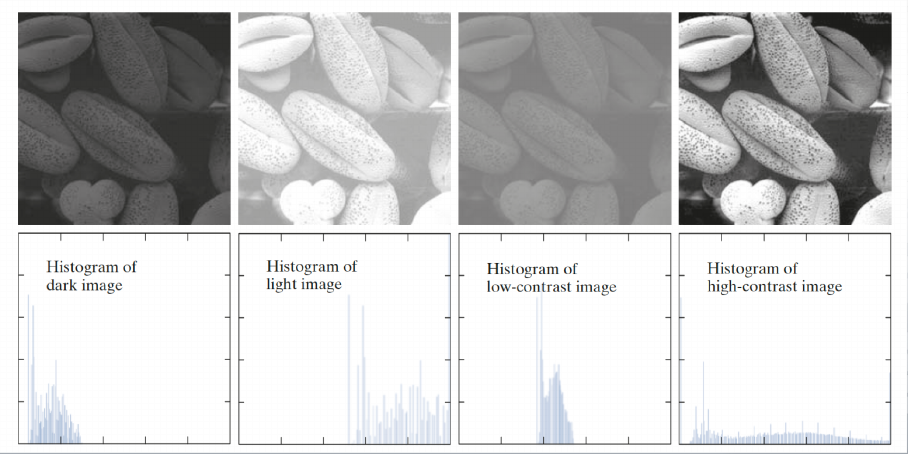
\includegraphics[width=.9\linewidth]{./img/histogram_example.png}
\caption{\label{Histogram_example}Example on the importance of histograms}
\end{figure}

importance of histogram that you can predict how will be your picture.
for example if the whole data is shifted to left so it will be dark picture.
if it is shifted to right it will be light image
if its in the middle so it will be low contrast image.
We can use histogram equalization to distribute the data in histogram to get high contrast as we will see in the next section.

\subsection{{\bfseries\sffamily TODO} Histogram equalization}
\label{sec:org6f143c5}
In this section we will talk about histogram equalization.

\uline{\textbf{importance}}


to get higher contrast of the picture.
we used python code [Histo.py] to represent the idea.
\begin{figure}[htbp]
\centering
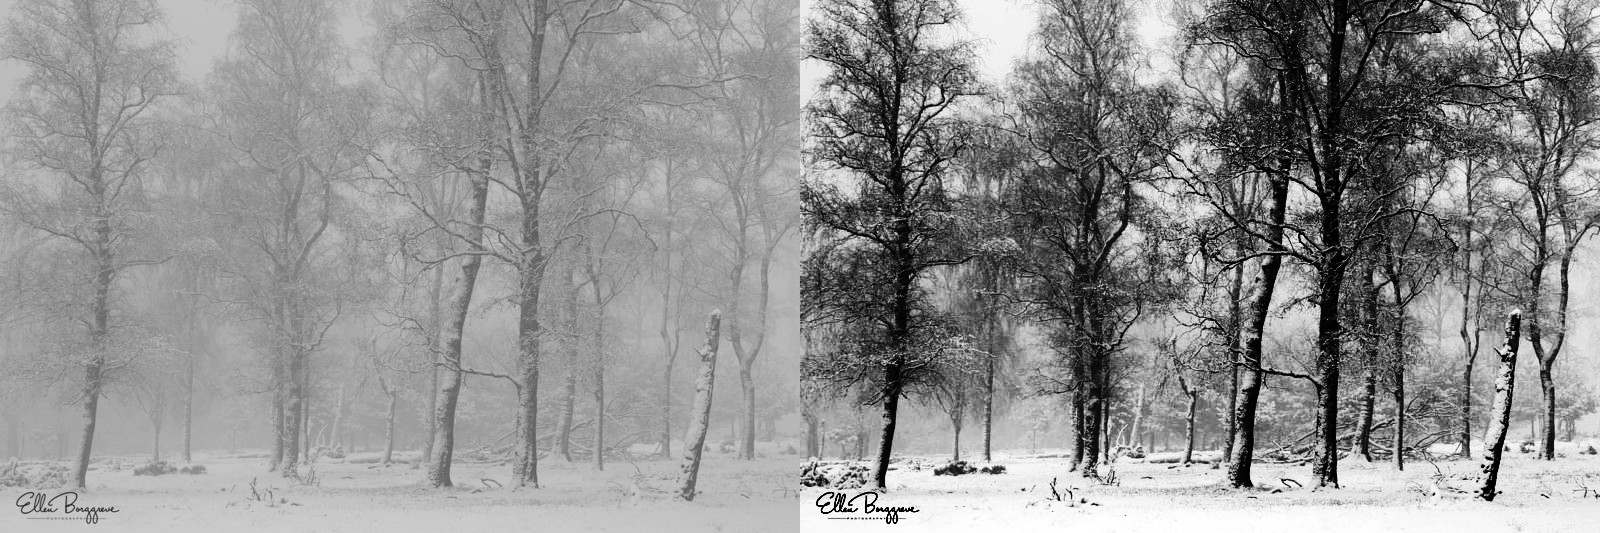
\includegraphics[width=.9\linewidth]{./img/res.png}
\caption{\label{result of histogram equalization}Example on the importance of histograms}
\end{figure}
\section{Fundamentals of spatial filtering}
\label{sec:orgac4bddb}
The name filter is borrowed from frequency domain processing where “filtering” refers to passing, modifying,
or rejecting specified frequency components of an image. For example, a filter that passes low frequencies is called a lowpass filter.
The net effect produced by a lowpass filter is to smooth an image by blurring it. We can accomplish similar smoothing directly on the
image itself by using spatial filters.
Spatial filtering modifies an image by replacing the value of each pixel by a function of the values of the pixel and its neighbors. If the
operation performed on the image pixels is linear, then the filter is called a linear spatial filter. Otherwise, the filter is a nonlinear spatial
filter. We will focus attention first on linear filters and then introduce some basic nonlinear filters. 
\subsection{linear filtering}
\label{sec:orgc529dd7}
kernel
\subsection{image padding}
\label{sec:org79289b4}
\subsection{correlation and convolution}
\label{sec:org5a6f019}
\subsection{Gaussian Filter}
\label{sec:orge41f316}
    A Gaussian filter is a linear filter. It's usually used to blur the image or to reduce noise. If you use two of them and subtract,
    you can use them for "unsharp masking" (edge detection).
    The Gaussian filter alone will blur edges and reduce contrast.
The Median filter is a non-linear filter that is most commonly used as a simple way to reduce noise in an image.
It's claim to fame (over Gaussian for noise reduction)
is that it removes noise while keeping edges relatively sharp.
I guess the one advantage a Gaussian filter has over a median filter is that it's faster because multiplying and adding is probably faster than sorting.
\end{document}
